\documentclass[
handout, 
aspectratio=169,
notes,
t]
{beamer}
% \setbeameroption{show notes on second screen=bottom} % Both
\setbeameroption{hide notes}
% \setbeamertemplate{note page}{\pagecolor{yellow!10}\insertnote}\usepackage{palatino}

\setbeamercovered{transparent}
\usepackage{tikz}
\usetheme{CambridgeUS}
% \usetheme{metropolis}
\usecolortheme{dolphin}
\setbeamertemplate{navigation symbols}{}
\setbeamertemplate{footline}[page number]
\setbeamertemplate{headline}

\usepackage{multicol}
\usepackage{natbib}
\usepackage{doi}
\usepackage{hyperref}
\hypersetup{colorlinks, allcolors=Blue}
\usepackage[normalem]{ulem}
\newcommand\WhileCC{\textit{\textbf{WhileCC}}}

\newcommand\SortOfSigma{\mathbf{Sort(\Sigma)}}
\newcommand\FuncOfSigma{\mathbf{Func(\Sigma)}}
\newcommand\VarOfSigma{\mathbf{Var(\Sigma)}}
\newcommand\TermOfSigma{\mathbf{Term(\Sigma)}}
\newcommand\StatementOfSigma{\mathbf{Stmt(\Sigma)}}
\newcommand\ProcOfSigma{\mathbf{Proc(\Sigma)}}
\newcommand\SIGMA{\mathbf{\Sigma}}


% -- Carrier sets
\newcommand\Reals{\mathbb{R}}
\newcommand\Nats{\mathbb{N}}
\newcommand\Bools{\mathbb{B}}
\newcommand\Rationals{\mathbb{Q}}
\newcommand\Integers{\mathbb{Z}}


\newcommand\algebraR{\mathcal{R}}
\newcommand\algebraB{\ensuremath{\mathcal{B}} }

\newcommand\real{\mathsf{real} }
\newcommand\nat{\mathsf{nat}}
\newcommand\bool{\mathsf{bool}}

\newcommand\dom{\mathbf{dom}} 

% -- Function Types
\newcommand\totalTo{\twoheadrightarrow}

% -- Function names
\newcommand\chooseOp{\mathsf{choose}}
\newcommand\returnOp{\mathsf{return}}

\newcommand\realZero{\mathsf{0_R}}
\newcommand\natZero{\mathsf{0_N}}

\newcommand\realOne{\ensuremath{\mathsf{1_R}} }
\newcommand\natOne{\ensuremath{\mathsf{1_N}} }
\newcommand\realMinusOne{\ensuremath{\mathsf{-1_R}} }
\newcommand\realPlus{\mathsf{+_R}}
\newcommand\realTimes{\mathsf{\times_R}}

\newcommand\realInv{\ensuremath{\mathsf{inv_R}} }
\newcommand\natSuc{\ensuremath{\mathsf{suc_N}} }
\newcommand\true{\mathsf{tt}}
\newcommand\false{\mathsf{ff}}
\newcommand\boolAnd{\mathrel{\mathsf{and}}}
\newcommand\boolOr{\mathrel{\mathsf{or}}}
\newcommand\boolNot{\ensuremath{\mathsf{not}} }
\newcommand\natEq{\mathrel{=_\mathsf{N}}}
\newcommand\natLess{\mathbin{<_\mathsf{N}}}
\newcommand\realEq{\mathbin{\ensuremath{\mathsf{eq_R}} }}
\newcommand\realLess{\mathbin{\mathsf{<_\mathsf{R}}}}
\newcommand\natPlus{\mathbin{+_\mathsf{N}}}
\newcommand\natTimes{\mathbin\times_{\mathsf{N}}}
\newcommand\abs[1]{{\lvert #1\rvert}}

\newcommand\ifff{\ \Longleftrightarrow \ }
\newcommand\then{\ \Longrightarrow \ }
\newcommand\Nbd{\mathbf{Nbd}}

\usepackage{amsmath, mathtools}
\usepackage{bbding}
\usepackage[dvipsnames]{xcolor}
\usepackage{edcomms}
\usepackage{wasysym}
\usepackage{pgfplots}
% \pgfplotsset{compat=1.18}

\title{\WhileCC-approximability and Acceptability of Elementary Functions}
\author{Fateme Ghasemi \and Dr. Jeffery Zucker\\
ghases5@mcmaster.ca \and zucker@mcmaster.ca}
\date{September 2025}
\titlegraphic{
\includegraphics[width=2cm]{mcmaster-logo.png}
}
\usefonttheme[onlymath]{serif}
\usepackage{etoolbox}
\setbeamertemplate{theorem begin}[normal font]

\let\originalnewtheorem\newtheorem
\RenewDocumentCommand{\newtheorem}{ommo}{%
  \originalnewtheorem{#2inner}{#3\thisthmnumber}
  \NewDocumentEnvironment{#2}{od()}
   {%
    \IfValueT{##2}{\renewcommand{\thisthmnumber}{ ##2}}%
    \IfValueTF{##1}{\begin{#2inner}[##1]}{\begin{#2inner}}%
   }
   {\end{#2inner}}
}
\newcommand{\thisthmnumber}{}
\newtheorem{ntheorem}{Theorem}

\begin{document}

\small
\maketitle

\section{Introduction}
    % \begin{frame}{Abstract Vs.\ Concrete Computation on $\Reals$}
    \begin{minipage}[t]{0.45\linewidth}
        \textbf{Concrete Models:}
        \begin{itemize}
            \item Depend on representation
            \item All equivalent to Grzegorczyk-Lacombe (GL)-computability
            \item
        \end{itemize}    
    \end{minipage}
    \pause
    \begin{minipage}[t]{0.45\linewidth}
        \textbf{Abstact Models:}
        \begin{itemize}
            \item 
        \end{itemize}
    \end{minipage}
\end{frame}
    \begin{frame}{Computability of Functions on $\Reals$}
\vspace{-1em}
    \pause
    \textbf{For total functions on $\Reals$}\pause, the following models of computation are equivalent \pause for all functions that are effectively locally uniformly continuous \citep{ComputableTotalFunctionsOnMetricAlgebras_JohnTuckerAndJeffZucker}:
    \begin{itemize}
        \item GL-computability,
        \item tracking computability,
        \item multipolynomial
        approximability, and
        \item \WhileCC-approximability.
    \end{itemize}
    \pause What about \textbf{\textcolor{Sepia}{partial}} functions? $1/x$, $\sqrt[n]{x}$, \ldots
    \pause
    
    \vspace{1em}
    \textbf{For partial functions on $\Reals$}, \citet{ModelOfCompForPartFunc_MingQuanFuAndJeffZucker} generalize effectively locally uniform continuity to \textbf{\textcolor{violet}{acceptability}} to get an equivalence.\\
    \pause
     \begin{exampleblock}{\textbf{\textcolor{BrickRed}{Problem}}}
        How general is this class of acceptable functions?
     \end{exampleblock}
     \pause
     \begin{exampleblock}{\color{OliveGreen}\textbf{Useful First Step Towards Solution}}
         Show that the elementary functions satisfy the acceptability conditions. 
     \end{exampleblock}
     \note[item]{Good Afternoon everyone, and thank you for being here for my talk.}
    \note[item]{Another special thank you to the organizers who set up this great series
    of talks, and also made it possible for some of us to attend virtually. }
    \note[item]{My name is Fateme and I recently graduated with my Master's from McMaster.}
    \note[item]{Today, I will be presenting the results from my Master's that was done
    under the supervision of Dr. Jeffery Zucker.}
    \note[item]{This is a continuation of the work done by Dr. Zucker and Dr. Tucker done 
    on computability on many-sorted algebras.}
    \note[item]{In this presentation, we will talk about computability on real numbers. For total functions, it's proven that when we talk about effective locally uniform continuous functions, these models of computation agree on the class of computable functions. The precise definition of effective local uniform continuity will not be given here since it's not relevant to the rest of this presentation.}
    \note[item]{But how about partial functions? There are many useful functions that we expect should be computable in any model.}
    \note[item]{There is a generalization of this concept of effective local uniform continuity, called acceptability, given by Fu and Zucker. Under this generalization, the same models are proven to be equivalent for partial functions. }
    \note[item]{Now the problem that we want to solve, is to see how general this acceptability condition is. We show that acceptability is at least general enough to include all elementary functions.}
\end{frame}


 
    % \begin{frame}{Problem}
    \begin{itemize}
        \pause \item Four models of computation for \textit{partial} functions on $\Reals$ are equivalent when assuming \textcolor{violet}{acceptability} of functions. 
        \pause \item How large is this class of acceptable functions?
    \end{itemize}
\pause \textbf{\textcolor{OliveGreen}{Solution}}\\
    \begin{itemize}
        \pause \item Show that the elementary functions satisfy the acceptability conditions. 
        % \pause Elementary functions are built up from \pause the variable $x$ \pause and constants for computable reals, \pause by applying (repeatedly) \pause the four fields operations,\pause $n$-th roots,\pause the exponential and trigonometric functions and their inverses.
        % \pause \item Compute the elementary functions  in one model (\WhileCC-approximability). 
        % \pause\item Prove that the elementary functions are \textcolor{violet}{acceptable} (and hence computable in all four).
    \end{itemize}
    
\end{frame}


\section{Background}
    % \begin{frame}{Background -- \WhileCC($\mathcal{R}$) Programming Language}
\setlength{\columnsep}{-0.5cm}
\begin{multicols}{2}
    \pause
        \fbox{
        \begin{tabular}{ll}
             algebra & $\algebraR$ \\
             carriers & $\Reals$, $\Nats$, $\Bools$ \\
             functions & $\realZero$, $\realOne$, $\realMinusOne$ : $\ \totalTo \mathbb{R}$ \\
              & $\realPlus$, $\realTimes$ : $\Reals\times\Reals\totalTo\Reals$\\
              & $\natPlus$, $\natTimes$ : $\Nats\times\Nats\totalTo\Nats$\\
              
              & $\realInv$ : $\Reals\to\Reals$ \\
              & $\natZero$ : $\ \totalTo \Nats$ \\
              & $\natSuc$ : $\Nats\totalTo\Nats$ \\
              & $\true$, $\false$ : $\ \totalTo\Bools$ \\ 
              & $\boolAnd$, $\boolOr$ : $\Bools\times\Bools\totalTo\Bools$ \\
              & $\boolNot$ : $\Bools\totalTo\Bools$ \\
              & $\natEq$, $\natLess$ : $\Nats\times\Nats\totalTo\Bools$ \\
              & \textcolor{violet}{$\mathsf{=_R}$, $\realLess$} : $\Reals\times\Reals \textcolor{violet}{\to{}}\Bools$ 
        \end{tabular}   
        }\\
        \edcomm{FG}{todo: put an arrow here pointing to the colored text, explaining partiality}
        % \vline{}
        \vfill\null
        \columnbreak
        \begin{itemize}
            \pause \item Variables from $\Reals$, $\Nats$, $\Bools$ 
            \pause \item Terms
                    \[ t^s ::= x^s\ \mid F(t_1^{s_1}, \ldots , t_m^{s_m}) \]
            \pause \item Statements
                \begin{align*}
                    S ::=& \ \mathsf{skip}\
                            \mid \mathsf{div}
                            \mid \bar{x} := \bar{t}
                            \mid S_1\ S_2\\
                            &\mid \mathsf{if}\ b \ \mathsf{then}\ S_1 \ \mathsf{else}\ S_2\ \mathsf{fi}\ \\
                            &\mid \mathsf{while}\ b\ \mathsf{do}\ S_0\ \mathsf{od}
                            \\
                            &\mid n:= \mathsf{choose\ } (z: \nat): P(z,\bar{t})
                \end{align*}
            \pause \item Procedures
                \begin{center}
                    $P$ ::= $\mathsf{proc} \ D\ \mathsf{begin}\ S\ \mathsf{end}$
                \end{center}
                    
        \end{itemize}
    \end{multicols}
\end{frame}

    
\begin{frame}{Background -- Acceptability}
\pause
    \begin{definition}[\textbf{\textcolor{violet}{Acceptability}}]
        A function $f:\Reals\to\Reals$ is \textbf{\textcolor{violet}{acceptable}} if there exists a sequence $X$ where:
        \begin{enumerate}
            \pause\item $X$ is an  \textbf{\textcolor{olive}{effective open exhaustion}} for $\dom(f)$, and
            \pause\item $f$ is  \textbf{\textcolor{brown}{effectively locally uniformly continuous w.r.t.\null{} $X$}}.
        \end{enumerate}
    \end{definition}
    % \vspace{-1.2em}
    \note[item]{First, let's start with defining acceptability formally. A function is called acceptable if its domain has an effective open exhaustion, and is effectively locally uniformly continuous with respect to that open exhaustion. Now, what are effective open exhaustions? and what does it mean for a function to be effectively locally uniformly continuous with respect to an effective open exhaustion? We will now define the concepts introduced here.}
\end{frame}
\begin{frame}{Background -- Effective Open Exhaustions}
\vspace{-1em}
\pause
\begin{definition}[\citep{ModelOfCompForPartFunc_MingQuanFuAndJeffZucker}]
        \pause A sequence $(U_1, U_2, \ldots)$ of open sets is called an \textbf{\textcolor{olive}{effective open exhaustion}} for an open $U\subseteq \Reals$ if 
        \pause \begin{enumerate}
                \item $ U = \bigcup_{l=0}^\infty U_l$, and
                \pause\item for each $l \in \Nats$,
                  $U_l$ is a finite union of non-empty open finite intervals $I_1^l, I_2^l,...,I_{k_l}^l $ whose closures are pairwise disjoint, and
                \pause\item for each $l \in \Nats$,
                   $\overline{U_l} = \bigcup_{i=1}^{k_l} \overline{I_i^l} \subseteq U_{l+1}$.
                \pause\item 
                for all $l$, the components $I_i^l$ that are intervals  building up the stage $U_l$, are \textit{rational} and \textit{ordered} i.e., $I_i^l = (a_i^l, b_i^l)$ for some $a_i^l, b_i^l \in \Rationals$ where $b_i^l < a_{i+1}^l$ for $i=1,...,k_l-1$, and
                \pause\item the map
                $l\mapsto ( a_1^l , b_1^l, ...,
                 a_{k_l}^l, b_{k_l}^l)$
                which delivers the sequence of stages $U_l = I_1^l\cup ...\cup I_{k_l}^l$ is recursive.
        \end{enumerate}
    \end{definition}
    \pause
    \begin{exampleblock}{\textbf{Example}}
        The sequence of open sets $(-1, 1), (-2, 2), \ldots, (-k, k), \ldots$
        is the standard effective open exhaustion for $\Reals$.
    \end{exampleblock}
    
   
    \note[item]{What is an effective open exhaustion? First of all, it's defined for open sets, so only open sets can have open exhaustions.}
    \note[item]{Also, it's a sequence of open sets that all unioned together should give us the original open set.}
    \note[item]{each element of the sequence, $U_l$,is called a stage, and is a union of a bunch of open intervals, the closures of which are disjoint.}
    \note[item]{the closure of each stage falls under the next stage}
    \note[item]{in each stage, the intervals are ordered and the endpoints are rational.}
    \note[item]{And the reason we call these effective is becuase the map delivering the endpoints of intervals in a stage should be recursive.}
    \note[item]{Now, as an example for an effective open exhaustion, consider the sequence here. In this example, each stage consists of a single interval and the union of all these sets covers the entire $\Reals$.}
\end{frame}
\begin{frame}{Background -- Effective Local Uniform Continuity}
    \begin{definition}[\citep{ModelOfCompForPartFunc_MingQuanFuAndJeffZucker}]
        A function $f$ on $U$ is \textbf{ effectively locally uniformly continuous \textbf{\textcolor{BrickRed}{w.r.t.\null{} an effective open exhaustion}}} $(U_n)_{n \in \Nats}$ of $U$, \pause if there is a recursive function $M:\Nats^2\totalTo \Nats$ such that for all $k,l \in \Nats$ and all $x,y \in U_l$:
        \[
        \abs{x-y}<2^{-M(k,l)} \then \abs{f(x)-f(y)}<2^{-k}
        \]    
    \end{definition}
    \note[item]{Now, we also needed effective local uniform continuity with respect to an effective open exhaustion.
    
    This is basically defined as standard uniform continuity, but over each stage. Also we require that the modulus of continuity $M$ is computable.}
\end{frame}
\section{Problem}
    \begin{frame}{Background -- Elementary Functions}
    \pause \vspace{-2em}
    \begin{minipage}[t]{0.48\linewidth}
        \begin{definition}[%Elementary functions,
                           \citep{OrdinaryDifferentialEquations_Morris_Tenenbaum_1985}]
            The \textbf{elementary functions} on $\Reals$  are partial functions defined by expressions built up from 
            \pause

            \kern-1ex
            \begin{itemize}
                \setlength\itemsep{-1pt}
                \item computable reals, and
                \item the variable $x$,
            \end{itemize}
            \kern-1ex
            \pause by applying (repeatedly) the basic operations below on elementary functions $f,g$:
            \pause
            \begin{itemize}
                \setlength\itemsep{-1pt}
                \item $(f+g)(x) = f(x) + g(x)$ 
                \item $(f\cdot g)(x) = f(x)g(x)$
                \item $\mathrm{div}_f(x) = \frac{1}{f(x)}$ \kern5em where $\frac{1}{0} =\ \uparrow$
                \item $\mathrm{root}_{n,f}(x) = \sqrt[n]{f(x)}$ \hfill where $0< n \in \Nats$
                \item $\ln_f(x) = \ln(f(x))$
                \item $\exp_f(x) = e^{f(x)}$
                \item $\sin_f(x) = \sin(f(x))$
                \item $\arcsin_f(x) = \arcsin(f(x))$
            \end{itemize}
        \end{definition}
    \end{minipage}
    \hfill
    \pause \begin{minipage}[t]{0.45\linewidth}
        \begin{exampleblock}{\textbf{\textcolor{BrickRed}{Problem}}}
            The domains of elementary functions are not all open!
        \end{exampleblock}
        \pause
        \begin{exampleblock}{\textbf{Solution: Modifications}}
            \pause
            \begin{itemize}
                \item We define $\sqrt[n]{x} = 0$ for $x < 0$ when $n$ is even.
                \pause \item We extend the definition of $\arcsin(x)$ to be $\frac{\pi}{2}$ for $x > 1$ and to be $-\frac{\pi}{2}$ for $x<-1$.
            \end{itemize}
        \end{exampleblock}
        \centering
        \visible<7->{
        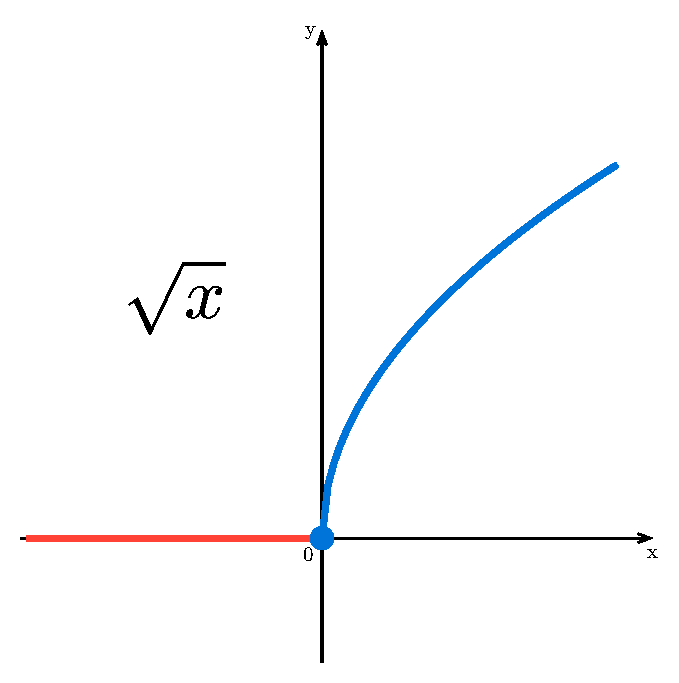
\includegraphics[width=0.35\linewidth]{sqrt.pdf}
        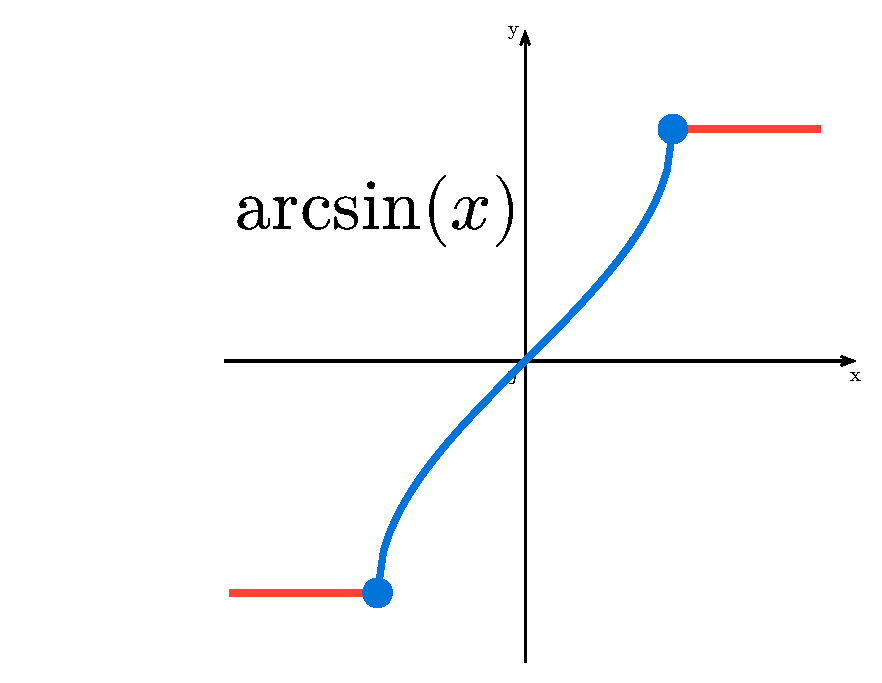
\includegraphics[width=0.35\linewidth]{arcsin.pdf}}
    \end{minipage}\kern-0.2em
    \note[item]{So the idea of the solution was to prove acceptability of elementary functions. Now that we have the definition of acceptability, we also need to review the definition of elementary functions.}
    \note[item]{
    Elementary functions are unary functions on $\Reals$, built up from the variable $x$ and compuatble reals, field operations, $n$th root, logarithm, exponential, and trigonometric functions. Note that addition and multiplication here are still unary functions.}
    \note[item]{Can we prove acceptability of elementary functions in their current forms? Looking more closely, we can see that not all the domains of the functions we just defined are open. So they cannot have effective open exhaustions for their domains.}
    \note[item]{What we can do to solve this, is to modify these functions to have open domains. Specifically we define even roots of a negative number to be $0$ and $\arcsin(x)$ to be defined as $\pi/2$ for $x>1$ and $-\pi/2$ for $x<-1$.}
\end{frame}
\section{Contributions}
    \begin{frame}{Contributions}
    \vspace{-1em}
    % \begin{exampleblock}
    {\color{gray}
    \textcolor{OliveGreen}{\textbf{Recall: Equivalence Theorem}, \citep{ModelOfCompForPartFunc_MingQuanFuAndJeffZucker}}\\
    For any \textcolor{violet}{acceptable function} $f:\Reals\to\Reals$ and any {effective open exhaustion} $X$ for $\dom(f)$, the following are equivalent:}

    \kern-1ex
        \begin{itemize}
            \setlength\itemsep{-3pt}\color{gray}
            \item $f$ is an $\alpha$-computable function.
            \item $f$ is \textcolor{BrickRed}{\WhileCC-approximable}.
            \item $f$ is GL-computable w.r.t. $X$.
            \item $f$ is effectively locally uniformly multipolynomially approximable w.r.t. $X$.
        \end{itemize}
    % \end{exampleblock}
    \pause 
    \begin{theorem}[\WhileCC-approximability Theorem]
        All elementary functions are \WhileCC-approximable.
    \end{theorem}
    \kern1ex
    \pause
    \begin{theorem}[Acceptability Theorem]
        All elementary functions are acceptable.
    \end{theorem}

    \kern1ex

    \pause
    \note[item]{In order to list the contributions, let us first recall the equivalence theorem by Fu and Zucker that we mentioned earlier. This theorem says that for any acceptable function, it's either computable in all of the computability models below, or is computable in none of them.}
    \note[item]{The second model of computability we listed here is an abstract model of computation on the reals. It is a simple while programming language featuring basic real operations, along with a countable choice operator that can choose natural numbers that satisfy a predicate. The CC in \WhileCC{} stands for countable choice. \WhileCC-approximability of a function basically means that we can write a program in \WhileCC{} that approximates that function arbitrarily close to the actual value.}
    \note[item]{Our work could be summarized in two theorems. The first theorem states that all elementary functions are computable in this \WhileCC-approximation model.}
    \note[item]{The second theorem uses the first one to prove that all elementary functions are acceptable.}
\end{frame}
\begin{frame}{Contributions}
    \vspace{-1em}
    {\color{gray}
    \textcolor{OliveGreen}{\textbf{Recall: Equivalence Theorem}, \citep{ModelOfCompForPartFunc_MingQuanFuAndJeffZucker}}\\
    For any \textcolor{violet}{acceptable function} $f:\Reals\to\Reals$ and any {effective open exhaustion} $X$ for $\dom(f)$, the following are equivalent:}

    \kern-1ex
        \begin{itemize}
            \setlength\itemsep{-3pt}\color{gray}
            \item $f$ is an $\alpha$-computable function.
            \item $f$ is \WhileCC-approximable.
            \item $f$ is GL-computable w.r.t. $X$.
            \item $f$ is effectively locally uniformly multipolynomially approximable w.r.t. $X$.
        \end{itemize}

    \kern1ex
    \begin{theorem}[\WhileCC-approximability Theorem]
        All elementary functions are \WhileCC-approximable.
    \end{theorem}

    \kern0.5ex
    \begin{theorem}[Acceptability Theorem: Part 1]
        The domain of any elementary function has an effective open exhaustion.
    \end{theorem}
    \pause
    
    \kern0.1ex
    \begin{theorem}[Acceptability Theorem: Part 2]
        Any elementary function is {effectively locally uniformly continuous} w.r.t.\null{} an effective open exhaustion for its domain.
    \end{theorem}
    \note[item]{Now this second theorem itself can be divided into two theorems based on the definition of acceptability. The first one states that for each elementary function, the domain has an effective open exhaustion. And the second one states that any elementary function is effectively locally uniformly continuous with respect to its domain.}
\end{frame}

    \begin{frame}{Challenges}
    \pause
    \begin{theorem}[\WhileCC-approximability Theorem]
        All elementary functions are \WhileCC-approximable.
    \end{theorem}
    \pause
    \begin{exampleblock}{}
    \center
    \large
        This is the easiest part, yet occupies about 30 pages of my thesis \ldots \smiley{} 
    \end{exampleblock}
    \note[itemize]{Talking about the challenges, the \WhileCC-approximability theorem is actually straightforward but super long. It's done by induction over the structure of elementary functions -- as one would expect. So this was not really a challenging part.}
\end{frame}
    
\begin{frame}{Challenges - \WhileCC-approximability Theorem - Background}
    \pause
    \footnotesize
    \begin{minipage}[t]{0.33\linewidth}
        \vspace{0.05em}
        \textbf{\color{Blue}{\WhileCC} Programming Language}
        {\textcolor{OliveGreen}{\textbf{ }}}
         \begin{itemize}
                \vspace{0.5em}
                \pause \item Terms
                \vspace{-0.5em}
                        \begin{align*}
                         t^s ::= x^s\ \mid F(t_1^{s_1}, \ldots , t_m^{s_m})
                        \end{align*}
                \vspace{-2.7em}
                \pause \item Statements
                \vspace{-0.5em}
                    \begin{align*}
                        &S ::=\\
                                &\ \mathsf{skip}\
                                \mid \mathsf{div}
                                \mid \bar{x} := \bar{t}
                                \mid S_1\ S_2\\
                                &\mid \mathsf{if}\ b \ \mathsf{then}\ S_1 \ \mathsf{else}\ S_2\ \mathsf{fi}\ \\
                                &\mid \mathsf{while}\ b\ \mathsf{do}\ S_0\ \mathsf{od}
                                \\
                                &\mid n:= \textcolor{BrickRed}{\mathsf{choose\ }} (z: \nat): P(z,\bar{t})
                    \end{align*}
                \vspace{-1.7em}
                \pause \item Procedures
                    \begin{center}
                        $P$ ::= $\mathsf{proc} \ D\ \mathsf{begin}\ S\ \mathsf{end}$
                    \end{center}
                        
            \end{itemize}
    \end{minipage}
    \begin{minipage}[t]{0.34\linewidth}
         \pause 
         \begin{center}
             \textbf{\color{Blue}Algebra $\algebraR$}
         \end{center}
         \begin{center}
            \fbox{
            \begin{tabular}{ll}
                 & $\Reals$, $\Nats$, $\Bools$ \\
                 & $\realZero$, $\realOne$, $\realMinusOne$ : $\ \totalTo \mathbb{R}$ \\
                  & $\realPlus$, $\realTimes$ : $\Reals\times\Reals\totalTo\Reals$\\
                  & $\natPlus$, $\natTimes$ : $\Nats\times\Nats\totalTo\Nats$\\
                  & {\color{BrickRed} $\realInv$ : $\Reals\ \to\ \Reals$} \\
                  & $\natZero$ : $\ \totalTo \Nats$ \\
                  & $\natSuc$ : $\Nats\totalTo\Nats$ \\
                  & $\true$, $\false$ : $\ \totalTo\Bools$ \\ 
                  & $\boolAnd$, $\boolOr$ : $\Bools\times\Bools\totalTo\Bools$ \\
                  & $\boolNot$ : $\Bools\totalTo\Bools$ \\
                  & $\natEq$, $\natLess$ : $\Nats\times\Nats\totalTo\Bools$ \\
                  & {\color{BrickRed} $\mathsf{=_{real}}$, $\realLess$ : $\Reals\times\Reals \ \to\ \Bools$} 
            \end{tabular}    
            }
        \end{center}
        
    \end{minipage}
    \begin{minipage}[t]{0.30\linewidth}
        \pause
        \begin{center}
             \vspace{1em}
         \end{center}            
            \begin{align*}
            \realInv(x) = &
                \begin{cases*}
                    1/x & if $x \neq 0$\\
                    {\color{BrickRed}\uparrow} & {\color{BrickRed}otherwise}
                \end{cases*}\\
            \mathsf{=_{real}}(x,y) = &
                \begin{cases*}
                    \false\ & if $x \neq y$\\
                    {\color{BrickRed} \uparrow\ }& {\color{BrickRed} otherwise}
                \end{cases*}\\
            \realLess(x,y) = &
                \begin{cases*}
                    \true\ & if $x<y$\\
                    \false\ & if $x>y$\\
                    {\color{BrickRed}\uparrow} & {\color{BrickRed} if $x=y$}\\
                \end{cases*}
            \end{align*}
        \setlength{\fboxsep}{0pt}
        \fbox{
        \begin{tabular}{l}
            The Semantics of a program $P$\\
            is denoted by a many-valued\\
        function $P^\algebraR$.
        \end{tabular}
        }
    \end{minipage}
    \note[itemize]{
    The functions commonly known as inverse, equality and order are not continuous.
    Since the concepts of \While{}-computability and \WhileCC-computability
    We are using here have been designed to make all expressed functions continuous on their domains \citep{ComputableFunctionsAndSemicomputableSetsOnManySortedAlgebras-TuckerAndZucker_Handbook_2001, AbstractVSConcreteComputationOnMetricPartialAlgebras_TuckerZucker_2004},
    the discontinuities in conventional models of equality, order, and inverse
    have been resolved by making the functions in $\mathcal{R}$ undefined there.
    }
        
\end{frame}


\begin{frame}{Challenges - \WhileCC-approximability Theorem - Background}
    \pause
    \begin{definition}[\WhileCC-approximability, \citep{ModelOfCompForPartFunc_MingQuanFuAndJeffZucker}]
\label{def::whileCC-approximable}
    A \WhileCC-procedure $P$ of type $\real\times\nat \to \real$ on $\algebraR$ is said to \textit{approximate} a function $f:\Reals\to\Reals$ iff for all $n\in \Nats$ and all $x\in \Reals$:
    \begin{itemize}
        \pause \item $x \in \dom(f) \then \emptyset \neq P^\algebraR(x,n) $ \pause  $\subseteq \Nbd(f(x), 2^{-n})$
            , and
        \pause \item $x \notin \dom(f) \then P^\algebraR(x)=\emptyset$
    \end{itemize}
    \pause where $\Nbd(y,r)$ has the standard definition of neighborhood on $\Reals$ i.e., \[\Nbd(y,r) = \{ z\in \Reals\ \mid \abs{y-z}<r \}.\]
\end{definition}

     \begin{exampleblock}{\textbf{\textcolor{OliveGreen}{Goal}}}
         Construct \WhileCC-procedures approximating elementary functions by induction
     \end{exampleblock}
     
     \begin{exampleblock}{\textcolor{BrickRed}{\textbf{Challenges:} Using comparison operators introduces undefinedness.}}
        \pause How do we \WhileCC-approximate ``piecewise'' functions?
     \end{exampleblock}

    \note[itemize]{Let us start with a more formal definition. We already defined the \WhileCC programming language earlier, but what does it mean for a function to be \WhileCC-approximable?\\
    The semantics for \WhileCC-programs is a multi-valued function. Now let's say $P$ is a \WhileCC-procedure with a real and a precision variable in \Nats as inputs. It is said to approximate a function $f$ on the reals if for any input in the domain of $f$, it gives us a nonempty set of values all close enough to $f(x)$. The definition of closeness (here, neighborhood) is the standard definition of neighborhood on the reals. }
\end{frame}

\begin{frame}{Challenges - \WhileCC-approximability Theorem}
    \begin{minipage}[t]{0.4\linewidth}
        \vspace{-2em}
        \begin{exampleblock}{\color{BrickRed}\textbf{Problem}}
            When defining piecewise functions, comparison makes a hole! 
        \end{exampleblock}
        \pause
        \vspace{0.75em}
        {\textbf{\color{MidnightBlue}Example: Even Root} \pause \textbf{\color{BrickRed} - First Attempt}\\}
        \footnotesize
        \vspace{-1em}
        \[ 
            \BLOCK{
            \PROC  \\
                \INDENT{
                \IN\ x:\real\ c:\nat}\\
            \BEGIN \\
                \INDENT{
                \IF x \realLess 0 \THEN \\
                    \INDENT{
                    \RETURN 0}\\
                \ELSE \\
                    \INDENT{
                    \RETURN \mathsf{Root}(x,c)}\\
                \FI \\

                }\\
            \END}\\
        \] 
        \pause
        \begin{flushright}
        % \includegraphics[width=.98\linewidth]{root.png}
            \vspace{-3em}
            \pause
            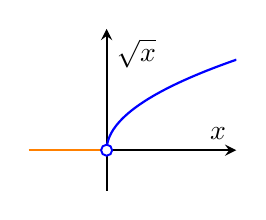
\begin{tikzpicture}
    \begin{axis}[
        width = 120,
        axis lines=middle,
        xlabel=$x$, ylabel=$\sqrt{x}$,
        samples=200,
        domain=-3:5,
        ymin=-1, ymax=3,
        xmin=-3, xmax=5,
        grid=both,
        thick, 
        xtick =\empty,
        ytick=\empty
    ]
    
    % Plot f(x) = 0 for x < 0
    \addplot[orange, thick, domain=-3:0] {0};
    
    % Plot f(x) = sqrt(x) for x > 0
    \addplot[blue, thick, domain=0:5] {sqrt(x)};
    
    % Open circle at (0,0) to indicate undefined
       \fill[color=white,draw=blue,line width=0.7pt] (axis cs:0,0) circle (2pt);
    
    \end{axis}
\end{tikzpicture}

        \end{flushright}
    \end{minipage}
    \begin{minipage}[t]{0.50\linewidth}
      
              
    \end{minipage}

\end{frame}


\begin{frame}{Challenges - \WhileCC-approximability Theorem}
    \begin{minipage}[t]{0.4\linewidth}
        \vspace{-2em}
        \begin{exampleblock}{\color{BrickRed}\textbf{Problem}}
            When defining piecewise functions, comparison makes a hole! 
        \end{exampleblock}
        \pause
        \vspace{0.75em}
         \begin{exampleblock}{\textbf{Solution}}
            \begin{itemize}
                \pause \item Find an overlapping interval where both pieces are defined
                \pause \item Use the nondeterminism of ``choose''  
            \end{itemize}
            % Assuming we have $\isCloseEnough(q,c,n) \implies \abs{\sqrt[c]{q}} < 2^{-n}$ 
            \pause
                       
        \end{exampleblock}     

        \pause
    \end{minipage}
    \begin{minipage}[t]{0.50\linewidth}
        % \vspace{-2em}
        \pause
        {
        \vspace{-1.5em}
        \center
        }
        \vspace{-1em}
        \scriptsize
         \[ 
            \BLOCK{             
                \PROC  \\
                    \INDENT{
                    \IN \ x:\real\ c:\nat \\
                    \AUX \chosenVal:\nat\ l:\real}\\
                \BEGIN \\
                    \INDENT{
                    l := \CHOOSE (q:\real) :
                                        \BLOCK{
                                        \isCloseEnough(q, c, n)} \\
                     \\
                    \chosenVal := \CHOOSE (k : \nat) :
                            \BLOCK{
                            \PROC \\
                                \INDENT{
                                \IN k:\nat\ x:\real}\\
                            \BEGIN \\
                                \INDENT{
                                \IF k \natEq 1 \THEN \\
                                    \INDENT{
                                    \RETURN 0<x}\\
                                \ELSE \IF k \natEq 2 \THEN \\
                                    \INDENT{
                                    \RETURN x<l}\\
                                \ELSE \\
                                    \INDENT{
                                    \RETURN \false}\\
                                \FI }\\
                            \END}\\
                    \IF \chosenVal \natEq 1 \THEN \\
                        \INDENT{
                        \RETURN \mathsf{Root}(x,c)}\\
                    \ELSE \IF \chosenVal \natEq 2 \THEN \\
                        \INDENT{
                        \RETURN 0}\\
                    \FI}\\
                \END}\\
            \] 
        \pause
        \begin{flushright}
        % \includegraphics[width=.98\linewidth]{root.png}
            \vspace{-8.5em}
            \pause
            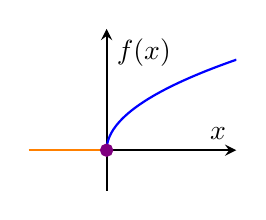
\begin{tikzpicture}
    \begin{axis}[
        width = 120,
        axis lines=middle,
        xlabel=$x$, ylabel=$f(x)$,
        samples=200,
        domain=-3:5,
        ymin=-1, ymax=3,
        xmin=-3, xmax=5,
        grid=both,
        thick, 
        xtick =\empty,
        ytick=\empty
    ]
    
    % Plot f(x) = 0 for x < 0
    \addplot[orange, thick, domain=-3:0] {0};
    
    % Plot f(x) = sqrt(x) for x >= 0
    \addplot[blue, thick, domain=0:5] {sqrt(x)};
    
    % Closed circle at (0,0) because both pieces agree
    \addplot[only marks, mark=*, mark size=2pt, violet] coordinates {(0,0)};
    
    \end{axis}
\end{tikzpicture}

        \end{flushright}
        
    \end{minipage}

\end{frame}
\section{Challenges}
    \begin{frame}{Challenges}
    \vspace{-1.5em}
    \begin{theorem}[Acceptability Theorem: Part 1]
        Let $f:\Reals\to\Reals$ be an elementary function. Then, $\dom(f)$ has an effective open exhaustion.
    \end{theorem}
    \pause
    \vspace{-2em}
    \begin{minipage}[t]{0.52\linewidth}
        \begin{exampleblock}{\textbf{\textcolor{Mahogany}{First attempt --  Strengthening:}}\\ \textcolor{Blue}{Elementary function constructions preserve
        the property that the domain has an effective open exhaustion.}}
            \begin{itemize}
            \setlength\itemsep{-2pt}
                \pause\item Base cases \Checkmark (e.g. $\sin(x)$)
                \pause\item Addition and multiplication \Checkmark (e.g. $(f+g)(x)$) 
                \pause \item Composition case has a counterexample:
                \pause \[ f(x) = \mathit{id}|_{(-1,1)}\text{ and } \pause  g(x) = 
                        \begin{cases*}
                            0 & if $-1\leq x \leq 1$ \\
                            1 & otherwise
                        \end{cases*}
                \]
                \pause$\dom(f)$ has an effective open exhaustion \Checkmark\\
                \pause$\dom(g)$ has an effective open exhaustion \Checkmark\\
                \pause$\dom(f\circ g) = [-1,1]$ has no open exhaustion \textcolor{Mahogany}{\XSolidBrush}
            \end{itemize}
        \end{exampleblock}
    \end{minipage}
    \hspace{1em}
    \pause
    \begin{minipage}[t]{0.44\linewidth}
        \begin{exampleblock}{\textbf{\textcolor{BrickRed}{Strengthened to proving \textbf{exhaustion reflection property}}}}
            \kern-1ex
            For any open set $U$ with an effective open exhaustion, $f^{-1}(U)$ has an effective open exhaustion.\\
            \pause
            Proof: By induction 
            \vspace{-0.5em}
            \begin{itemize}
                \setlength\itemsep{-5pt}
                \pause\item Base cases \Checkmark
                \pause\item Composition \Checkmark 
                \pause \item Addition and multiplication \textcolor{Mahogany}{\XSolidBrush}
            \end{itemize}
        \end{exampleblock}
        \vspace{-1em} \pause
        \begin{exampleblock}{\textbf{\textcolor{OliveGreen}{Adding decomposition of $+$ and $\cdot$}}}
        \vspace{-0.5em}
        $(f+g)(x) = f(x)+g(x)$ is composed of
        \vspace{-0.5em}
        \begin{itemize}
            \setlength\itemsep{-4pt}
            \item $\mathit{Add}(x,y) = x + y$,
            \item $\mathit{Add}(x,y) = x + y$,
            \item $(f\times g)(x,y) = (f(x),g(y))$, 
            \item $\mathit{Diag}(x) = (x,x) \qquad$ 
        \end{itemize}
        \end{exampleblock}
    \end{minipage}
    \note[itemize]{
    \footnotesize One of the actual interesting challenges was the first part of the acceptability theorem. What we needed to prove was that for any elementary function, the domain has an effective open exhaustion. Our first attempt was of course proof by induction. The base cases, addition, and multiplication are all trivial. But the composition case does not work. Let us consider the two functions $f$ and $g$ here. $f$ is just the identity function, but its domain is restricted to $(-1,1)$. This is just an interval with rational endpoints, and hence has an obvious effective open exhaustion. The domain of $g$ is the reals and has the standard effective open exhaustion. But when we compose the two together to get $f\circ g$, the domain of $f\circ g$ is $[-1,1]$ which is no longer open. So in order to prove the theorem by induction, we had to strengthen the theorem into this exhaustion-reflection property here. This property says if we have an open set with an effective open exhaustion, then the pre-image of that set should have an effective open exhaustion as well. Proving this new property for all the elementary functions using induction, again base cases go through easily. Composition is made easy. But this time addition and multiplication are the problem. The idea that we used here, is to deconstruct the addition and similarly multiplicaion into the following functions and prove the exhaustion-reflection property for each of these functions. Note that before this deconstruction we did not deal with non-unary functions, but in order to use this method, we had to generalize the definition of an effective open exhaustion to more than one dimension, requiring us to also prove the exhaustion-reflection property for a generalized version of composition. }
\end{frame}
    \begin{frame}{Interesting results - Acceptability Theorem }
    \pause
    \begin{minipage}[t]{0.45\linewidth}
    \vspace{-2.5em}
    \begin{theorem}[Reducing Exhaustion-reflection to to a Decision Procedure]
        A function $f:\Reals^n \to\Reals^m$ is exhaustion-reflecting, if we can decide for any $m$-cube $Q_m$ whether an arbitrary rational closed $n$-cube is completely contained in $f^{-1}(Q_m)$.
    \end{theorem}
    \pause
    \begin{itemize}
        \item This is very useful for proving the exhaustion-reflection property for the addition and multiplication case.
    \end{itemize}

    \end{minipage}
    \begin{minipage}[t]{0.54\linewidth}
        \center
        \pause
        \vspace{-1em}
        \color{Mahogany}
        \textbf{The process of building an effective open exhaustion}
        \vspace{-1em}
        \begin{flushright}
            \pause
            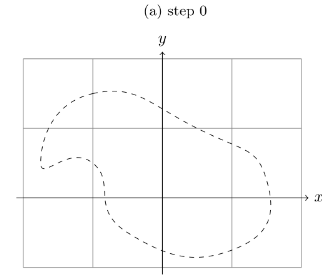
\includegraphics[width=0.48\linewidth]{tikz/step0.png}
            \pause
            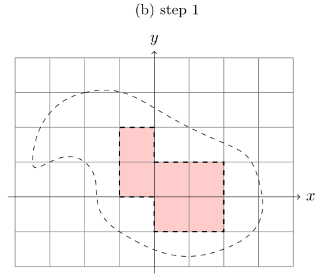
\includegraphics[width=0.48\linewidth]{tikz/step1.png}
            \pause
            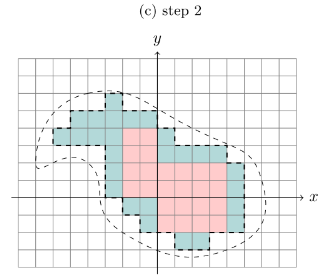
\includegraphics[width=0.48\linewidth]{tikz/step2.png}
            \pause
            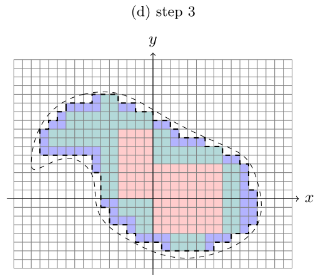
\includegraphics[width=0.48\linewidth]{tikz/step3.png}
        \end{flushright}
    \end{minipage}
\end{frame}
    \begin{frame}{Result 2}
    \pause
    \vspace{-1.5em}
    \begin{ntheorem}[Acceptability Theorem: Part 2](2.2)
        Any elementary function is effectively locally uniformly continuous \textbf{\textcolor{BrickRed}{w.r.t.\null{} an effective open exhaustion}} for its domain.
    \end{ntheorem}
    \pause
    \vspace{-0.5em}
    \begin{exampleblock}{\color{OliveGreen}\textbf{(We prove that this is) equivalent to proving:}}
        Any elementary function has a local continuity witness.
    \end{exampleblock}
    \pause
    \vspace{-0.5em}
    \begin{definition}[Local continuity witness]
        Let $f:\Reals\to\Reals$. A recursive function $N:\Rationals\times\Rationals\times\Nats\to\Nats$ is called a \textbf{local continuity witness} for $f$\index{local continuity witness} iff for any $a,b\in\Rationals$ with $[a,b]\subseteq\dom(f)$ and $k\in\Nats$, we have
        \[ 
            \forall x,y \in (a,b) \quad \abs{x-y}<2^{-N(a,b,k)} \then \abs{f(x)-f(y)}<2^{-k}.
        \] 
    \end{definition}
    \vspace{-0.5em}
    \pause
    \begin{theorem}
        Let $f:\Reals\to\Reals$ be \WhileCC-approximable and monotone on its domain. 
        Then $f$ has a local continuity witness.
    \end{theorem}
    \pause
        {\textbf{\textcolor{OliveGreen}{The notion of effective local uniform continuity is independent
                of effective open exhaustion.}}}
    \note{Now we need to prove effective local uniform continuity of any elementary function with respect to its domain's effective open exhaustion.
    It is easier for our purposes to use an equivalent definition.
    Intuitively, the existence of a local continuity witness is similar to effective local uniform continuity w.r.t. an effective open exhaustion, except that, instead of the recursive function parameterized by the stage number, it is parameterized by the endpoints of an interval in its domain.\\
    The proof for both base cases and induction steps use the \WhileCC-approximability theorem (proved earlier) to overapproximate how much the value of a function changes within an interval in the domain.
    The composition case is mindnumbingly technical, so we won't go into the details here.
    %The composition case is a little bit trickier, since we need to prove that for any elementary function $f$ and open set $U$ with an effective exhaustion, we have some effective way of computing the stage number of $f(x)$ for any $x$ in an interval in some stage $l$ of an effective open exhaustion for $f^{-1}(U)$. But I won't go into the details here.
    }

\end{frame}
\section{Summary and Future Work}
    \begin{frame}{Takaways}
    \pause
    \begin{itemize}
        \item We presented an \textbf{alternative characterization} of acceptable functions \pause using the \textbf{local continuity witness} concept.
    \end{itemize}
\end{frame}

    \begin{frame}{Summary}
    We proved that:
    \pause
    \begin{itemize}
        \item all elementary functions are \WhileCC-approximable.
        \pause \item all elementary functions are acceptable.
    \end{itemize}
     \pause We also 
    \begin{itemize}
         \item  presented an \textbf{alternative characterization} of acceptable functions \pause using the \textbf{local continuity witness} concept, and
         \item found a few useful tricks along the way for implementing approximations of piecewise functions.
    \end{itemize}
\end{frame}

    \begin{frame}{Future Work}
    \pause
    \textbf{Questions left unanswered:}
    \begin{itemize}
        \pause \item Are non-unary elementary functions acceptable? \\
        \pause A generalization of acceptability in arbitrary metric spaces is given by \citet{AbstractVSConcreteComputationOnMetricPartialAlgebras_TuckerZucker_2004}.              
        \pause\item Can we extend the equivalence theorem in \citet{ModelOfCompForPartFunc_MingQuanFuAndJeffZucker} to acceptable partial functions of type $\Reals^m\to\Reals$? 

        \pause \item What functions are \WhileCC-approximable but not While*-approximable \citep{ComputationByWhileProgramsOnTopologicalPartialAlgebras_TuckerAndZucker}?
    \end{itemize}
    \pause \textbf{Conjecture:}
    \begin{itemize}
        \item All partial unary \WhileCC-approximable functions are acceptable.
    % \textbf{More Questions:}
    \begin{itemize}
        \pause \item \textbf{If the conjecture holds}, are \emph{non-unary} \WhileCC-approximable functions acceptable?
        \pause \item  \textbf{If not}, what is a model of computation that characterizes exactly the class of acceptable functions?
    \end{itemize}
    \end{itemize}
    \pause \textbf{Currently working on:}
    \begin{itemize}
        \pause \item {\color{olive}Formalizing the concept of \WhileCC-approximability and the aforementioned proofs in Lean.}
    \end{itemize}
\end{frame}

    \begin{frame}{References}
    \bibliographystyle{plainnat}
    \bibliography{refs}
\end{frame}
    \begin{frame}
    \vspace{1.2in}
    \center \textcolor{Blue}{\huge{A HUGE Thank you!}}
\end{frame}
\end{document}
